\chapter{Experiments}
\label{cha:Experiments}

\section{Evaluation metrics}

\subsection{success\_rate}
The primary metric of evaluation for the developed agents is the $success\_rate$. The $success\_rate$ is defined as the ratio of successful episodes to the total number of episodes. An episode is considered successful if the agent passes through all three goals within the time limit \ref{time_limit}. Collisions of the agent do not disqualify an episode from being succesful, as long as the agent passes all goals.

\subsection{goal\_completion\_rate}

The $goal\_completion\_rate$ is defined as the ratio of passed goals to the total number of goals in the episodes. The $goal\_completion\_rate$ is a more fine-grained metric than the $success\_rate$. However the two metrics are closely related as a high $success\_rate$ implies a high goal\_completion\_rate. The major advantage of the $goal\_completion\_rate$ is that it can used to measure the progress of an agent during training more accurately. 
The $goal\_completion\_rate$ would increase when the agent is able to pass more goals on average, whereas the $success\_rate$ would only increase when the agent is able to pass all goals in an episode more often. The $goal\_completion\_rate$ captures learning progress earlier in training. This behaviour can be observed in training runs, shown in \ref{fig:success_rate_vs_goal_completion_rate}.


\begin{figure}
    \centering
    \subfigure[success\_rate]{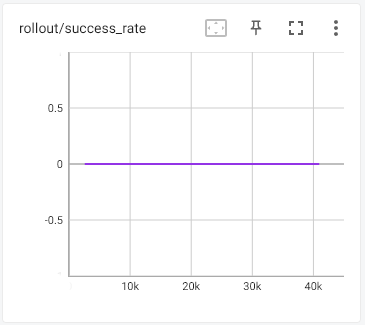
\includegraphics[width=0.3\textwidth]{Bilder/metrics/sr_vs_gcr_success_rate.PNG}}
    \subfigure[goal\_completion\_rate]{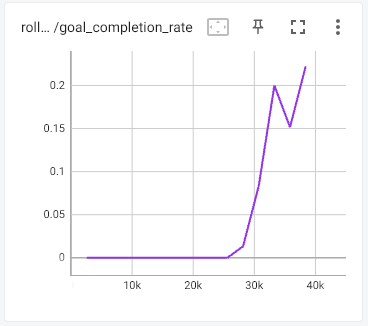
\includegraphics[width=0.3\textwidth]{Bilder/metrics/sr_vs_gcr_goal_completion_rate.PNG}}
    \caption{Difference in success rate and goal completion rate during early stages of training.}
    \label{fig:success_rate_vs_goal_completion_rate}
\end{figure}
% diese Bilder funktionieren nur für frühe Episoden, später sind die Werte sehr gleich


\section{Basic evaluation algorithm}
\label{sec:eval_model_track}

This section explains most important component of the evaluation algorithms. It explains how the agent's performance is evaluated on a specific light and difficulty setting. This basic component is widely used in the following tests.

The agent is evaluated by running a fixed number of episodes for the specific light and difficulty settings. The amount of episodes that the agent is evaluated on is defined by the config parameter $n\_eval\_episodes$. As described in \ref{cha:env_description}, each difficulty setting includes a number of unique tracks. Furthermore the initial starting position/rotation is parameterized by the config parameter $spawn\_point$.
The tracks and starting positions for the agent are generated by the algorithm shown in \ref{fig:generate_track_rotation}. The algorithm divides the random interval specified by the spawn point parameter into $n\_eval\_episodes$ equal parts. These spawn rotations are then each assigned a track in repeating order.
This algorithm ensures that the agent is evaluated on the full range of unique tracks and spawn points.
It also makes the evaluations comparable, as the same combinations of tracks and spawn points are used for each agent evaluation.

The evaluation algorithm initializes $n\_eval\_episodes$ environments with the specified light settings. The obstacles and agents are then placed in the environments according to the generated map and rotation pairs. The evaluation episodes are started and the agents act in their environment until their episodes are terminated. The $success\_rate$ and other metrics are calculated from the terminated episodes.



\section{Standard evaluation runs}

The agent is evaluated on every combination of light and difficulty settings. The $success\_rate$ metric is collected for each combination of light and difficulty settings separately. The collected $success\_rates$ are then averaged to produce aggregate $success\_rates$ for each light setting and difficulty setting. The 3 light and difficulty settings result in a total of 9 evaluated combinations and $success\_rates$. A total of 7 aggregate $success\_rates$ are computed, 3 for each light setting and 3 for each difficulty setting. The final aggregate is the $total\_success\_rate$, the average of all 9 collected $success\_rates$. 
The $total\_success\_rate$ is used to determine the overall best agent and model.


\begin{table}
\begin{center}
\resizebox{\textwidth}{!}{%
\begin{tabular}{|| c | c | c | c | c ||} 
    \hline
    \makecell{} & bright & standard  & hard & \makecell{aggregate \\ success\_rates} \\ [0.5ex] 
    \hline\hline
    \makecell{easy} &  success\_easy\_bright & success\_easy\_standard & success\_easy\_dark & success\_easy \\ 
    \hline
    \makecell{medium} &  success\_medium\_bright & success\_medium\_standard & success\_medium\_dark & success\_medium \\ 
    \hline
    \makecell{hard} &  success\_hard\_bright & success\_hard\_standard & success\_hard\_dark & success\_hard \\ 
    \hline
    \makecell{aggregate \\ success\_rates}  & success\_bright & success\_standard & success\_dark & total\_success\_rate \\
    \hline
\end{tabular}}
\end{center}
\caption{Collected and aggregate success\_rate metrics}
\label{table:success_rates_system}
\end{table}




\subsection{Deterministic check}

The PPO policy produces an action distribution when given an input observation. The action distribution is sampled to obtain an action for the agent to execute in the environment. The distribution can be sampled deterministically or non-deterministically. Deterministic sampling returns the most likely action, indicated by the mean of the distribution. Non-deterministic sampling returns a sample from the distribution according to the distribution's probabilities. This results in different output actions for the same observations. The PPO policy uses non-deterministic sampling during training to explore the action space. 

While the exploration caused by non-deterministic sampling is beneficial during training, it could be detrimental during evaluation. This exploration could lead the agent to take actions that are not optimal for the given observation and result in a lower $success\_rate$. Non-deterministic sampling can also be used during evaluation to reduce overfitting. This has been used in the Atari paper \autocite{atari} and the human-level control paper \autocite{human_level_control}. The environments examined in these papers are deterministic with identical starting states. Therefore a deterministic policy would result in identical results for the individual evaluation episodes.
Due to the difference in environment properties between the JetBot environment and the Atari environment, it is not clear if deterministic or non-deterministic sampling is better for the JetBot environment. The deterministic check evaluates the agent with deterministic and non-deterministic sampling to determine if the agent's performance is affected by the sampling method. 
The better sampling method is determined experimentally. It is then used for all agent evaluations.

% atari.pdf and human_level_control.pdf uses epsilon greedy during evals (their environment is deterministic, thus using a deterministic policy would result in the same results for every episode)


% default we use non deterministic, as that has shown (slightly) better results and is also used by atari paper



\subsection{Identical start condition Test}

% TODO the policy is also non-determinsitic during the eval runs, so the purpose of this test is a bit different (first paragraph)
The environment is simulated in Untiy and was described in \ref{cha:env_description} to not be fully deterministic. This means identical actions in identical environments could result in different outcomes. These changes are small, such as changes to a few pixels in the agent camera. However these small changes might result in different agent actions. These actions further influence the environment and following actions. This means that episodes with identical starting conditions could result in different outcomes. This could be problematic when evaluating the agent, as the agent's performance could be influenced by the environment's randomness. 

The identical start condition test evaluates the agent on multiple episodes with identical starting conditions. The episode results are analysed to see if the policy is consistent when given identical starting conditions. If the policy is inconsistent given identical starting conditions the evaluation results according to \ref{sec:eval_model_track} are not reliable. The evaluation algorithm described in \ref{sec:eval_model_track} evaluates the agent on a series of different starting conditions, each starting condition is unique and only evaluated once.

This test runs multiple episodes with identical start conditions and analyses the episodes. The episode results are characterized and grouped. The groups are then analysed to determine if the agent's performance is consistent given identical starting conditions. A low number of groups indicates that the agent's performance is consistent. Ideally there is only one group that all episode results belong to.
The episode results are characterized by the endEvent, collision and the three goals' completion.



\subsection{Fresh Observation Test}

In the standard reinforcement learning algorithms each step transition results in a new observation that represents the environment's new state. Calls to the Unity environment and the step transitions in the environment take time. In order to speed up the training process the step calls to the simulated environment have been implemented in a non-blocking way. This means the step calls return before the entire step transition has been completed. The observation after the step transition is not yet available when the call returns. The observation returned by the step call is the observation of the environment at the beginning of the step transition. This observation does not capture the changes that have occurred in the environment during the step transition. The full changes are then visible to the agent after the next step has completed. 

The option $use\_fresh\_obs$ controls what observations the policy uses to produce the next actions. If $use\_fresh\_obs$ is set to false, the observation returned by the last step call is used. If $use\_fresh\_obs$ is set to true, a new observation is requested from the Unity simulation.

The fresh observation test evaluates a trained policy with both $use\_fresh\_obs$ settings to determine if the agent's performance is influenced by the freshness of the observations. The trained policy used one setting of the $use\_fresh\_obs$ parameter during training. The test shows if there is a difference in the agent's performance when using the other setting. The test evaluates the agent on light and difficulty settings following the evaluation algorithm described in \ref{sec:eval_model_track}.


% ## fresh obs better than nonfresh obs
 
% ### models trained on nonfresh obs

% fresh obs are better than non-fresh obs

% ### models trained on fresh obs

% TODO can we train in use_fresh_obs mode? if so, then we should do that
% this removes the need to do this test and explain this

% we can copy this section somewhere else to highlight the learning/development process


\subsection{policy timestepLength generalization}

policy timestepLength generalization 

what happens to a model trained on fixedTimestepsLength when it is evaluated with a shorter/longer/unrestricted fixedTimestepsLength


\subsection{JetBot generalization}

There are two versions of the agent in simulation. The DifferentialJetBot has two front wheels that are accelerated independently for steering. The FourWheelJetBot angles its front wheels for steering. The differences can result in different agent movement for the same acceleration inputs. One specific version of the agent is used during training, the agent movement has an influence on the developed policy.
A policy trained on the DifferentialJetBot might not generalize well to the FourWheelJetBot and vice versa. The JetBot generalization test evaluates the trained policy on both JetBot versions to determine if the policy generalizes well. The test evaluates the agent on the different difficulty levels following the evaluation algorithm described in \ref{sec:eval_model_track}.



